\chapter{Circuito sináptico: diseño}

En este capítulo se va a tratar el diseño de un circuito neuromórfico. El objetivo principal es el diseño de un circuito capaz de replicar el comportamiento de una sinapsis neuronal, es decir, un circuito que emule la transmisión de un impulso nervioso de una neurona a otra. La función de un circuito sináptico es la de trasladar los pulsos de tensión presinápticos de la neurona transmisora, en corrientes postsinápticas inyectadas en la membrana plasmática de la neurona receptora. 

Para ello, el uso de circuitos que operen en la región subumbral se hace imprescindible, dado a su bajo consumo de potencia, así como de su característica exponencial, que los hace únicos para este tipo de funciones.

\section{Región subumbral (weak-inversion)}

A los modos de operación de un transistor MOSFET hasta ahora conocidos, hay que añadir uno más: el modo subthreshold, weak-inversion o subumbral. Este modo de operación se produce cuando:

\begin{equation}
0<V_{GS}<V{th}
\end{equation}

Se caracteriza por el hecho de que la mayoría de los portadores mayoritarios han sido expulsados de la superficie. La densidad de portadores minoritarios aumenta respecto a la distancia al substrato. Son estos portadores minoritarios las únicas cargas disponibles sobre la superficie del transistor, y por tanto, al aplicar una tensión por pequeña que sea entre el drenador y la fuente, estos se mueven por difusión, dando lugar a una corriente a través del transistor, tal y como se describe en\cite{vittoz2006origins}.

Además, se puede describir esta corriente mediante la ecuación:

\begin{equation}
I_D=I_{D0}e^{\frac{V_G}{nV_T}}(e^{\frac{-V_S}{V_T}}-e^{\frac{-V_D}{V_T}})
\end{equation}
\noindent
en la que todas las tensiones están referidas a la tensión del substrato. De esta forma, para el caso en el que el substrato esté conectado con la fuente, queda:

\begin{equation}
I_D=I_{D0}e^{\frac{V_{GS}}{nV_T}}(1-e^{\frac{-V_{DS}}{V_T}})
\end{equation}

Además, en cuanto que $V_{DS}\approx >2 V$, el término $e^{\frac{-V_{DS}}{V_T}}\approx 0$, y por tanto, el término $1-e^{\frac{-V_{DS}}{V_T}}\approx 1$. Si además definimos $\kappa =1/n$, como el separador del canal\footnote{$\kappa =\frac{C_{OX}}{C_{OX}+C_D}$, siendo $C_{OX}$ la capacidad de la capa de óxido, y $C_D$ la capacidad de la capa de agotamiento}, queda:

\begin{equation}
I_D=I_{D0}e^{\frac{\kappa V_{GS}}{V_T}}
\end{equation}

Se ha llegado en la ecuación 5.4, a una expresión compacta y simplificada para la corriente que circula por el transistor en la región de operación subumbral.

\section{Circuitos translineales y en modo corriente}

La palabra translineal como característica propia de un circuito electrónico fue por primera vez acuñada por Barrie Gilbert en \cite{gilbert1996translinear}. Este término hacía referencia al hecho de que la transconductancia de un transistor bipolar es linealmente proporcional a su corriente de colector. En este tipo de circuitos se observaban comportamientos distintos a los circuitos convencionales que se llevaban fabricando hasta la época, entre estos destaca el hecho de que estos circuitos estaban formados por celdas cerradas que contenían al menos dos uniones base-emisor, pero en otros casos cuatro, seis o incluso más. Las variables que controlaban el circuito eran corrientes, y es por esto que se decía que estos circuitos operaban en modo corriente. Las tensiones entre las diferentes partes del circuito dejaron de ser importantes, pasaron a un segundo plano. Además, debido a la baja tensión de alimentación, aumentó el ancho de banda de estos circuitos ya que el impacto de las uniones colector-base y colector-substrato en las frecuencias de corte desaparecieron. A diferencia del resto de circuitos conocidos hasta entonces, estos presentaban una altamente predecible relación entre sus variables de entrada y salida, a pesar de operar a alta frecuencia. Finalmente, uno de sus mayores funcionalidades era la capacidad para realizar operaciones algebraicas de todo tipo, cuadrados, raíces, operaciones vectoriales, etc, en cuestión de unos pocos nanosegundos. 

El principio de translinealidad dice que: {\bf{\it En un bucle cerrado que contenga un número par de uniones, de forma que haya el mismo número de uniones en el sentido de las agujas del reloj como de uniones en sentido contrario al de las agujas del reloj, y siempre y cuando no haya ningún generador de tensión dentro de este bucle, el producto de las densidades de corriente en uno de los sentidos es igual al producto de las densidades en el otro de los sentidos}}. De forma matemática lo podemos expresar como: $$\prod_{CW}J=\prod_{CCW}J$$ Es fácil darse cuenta de que gracias a esta igualdad podemos diseñar circuitos capaces de multiplicar, dividir, hacer raíces cuadradas y multitud de operaciones algebraicas en nanosegundos, por lo que la capacidad de estas celdas es comparable a la de un microprocesador. Solo hay que tener en cuenta que el resultado de la operación para el que diseñemos la celda en concreto será obtenido en forma de corriente a la salida del circuito.

Este comportamiento se puede extender también a los transistores MOS, siempre y cuando estos se encuentren en la región subumbral de funcionamiento, descrita anteriormente. Es por esto que para el diseño de circuitos sinápticos que se ha ido realizando desde las dos últimas décadas del siglo pasado hasta hoy, se ha hecho uso de estos circuitos translineales. Las ventajas de utilizar corrientes de valores tan pequeños en el caso de los tansistores MOS debido a su especial polarización tiene una ventaja única: un consumo de potencia mínimo.

\section{Circuito propuesto}

A continuación se va a describir el diseño y análisis del circuito propuesto. Primero se mostrará un modelo simplificado del circuito para ir paso a paso añadiendo complejidad al análisis, hasta llegar al circuito final.

\subsection{Modelo inicial}

En la figura \ref{Inicial} se muestra el esquemático del circuito simplificado inicial. En éste se usan fuentes de corriente ideales, que posteriormente serán sustituídas por sus modelos correspondientes. Este primer modelo servirá por tanto, para analizar el circuito de una forma más sencilla, así como para conocer qué papel juega cada uno de los parámetros que en él aparecen en la salida que se obtenga.

	\begin{center}
		\includegraphics[width=10cm]{Imagenes/Sinaptico/Inicial.eps}
    		\captionof{figure}{Esquemático del circuito inicial}\label{Inicial}
	\end{center}	

El objetivo ahora es obtener el valor de $I_{out}$. Para ello se aplicará el método de las corrientes en los nodos. El primer nodo que se analizará es el que une los dos Mosfet de canal N con la fuente de corriente $I_{in}$. 

\subsubsection{Nodo $S_1$}
En este nodo, debe cumplirse que:

\begin{equation}
I_{in}=I_g+I_d
\end{equation}

Ahora veamos cuál es la ecuación que describe a cada uno de los elementos que conforman esta ecuación. Es importante recalcar que la expresión que se usará para obtener el valor de estas corrientes es la deducida en el apartado anterior de esta memoria en la ecuación 5.4. 

$$I_g=I_0e^{\frac{\kappa}{V_T}(V_g-V_{S1})}=I_0\frac{e^{\frac{\kappa V_g}{V_T}}}{e^{\frac{\kappa V_{S1}}{V_T}}}$$

$$I_d=I_0e^{\frac{\kappa}{V_T}(V_c-V_{S1})}=I_0\frac{e^{\frac{\kappa V_c}{V_T}}}{e^{\frac{\kappa V_{S1}}{V_T}}}$$

Ahora, se puede obtener la relación $I_g/I_{in}$ haciendo uso de la ecuación 5.5:

$$\frac{I_g}{I_{in}}=\frac{I_g}{I_g+I_d}=\frac{e^{\frac{\kappa V_g}{V_T}}}{e^{\frac{\kappa V_C}{V_T}}+e^{\frac{\kappa V_g}{V_T}}}$$

De la ecuación 5.5, obtenemos también la relación:

$$\frac{I_d}{I_{in}}=1-\frac{I_g}{I_{in}}$$

A partir de los resultados obtenidos, se llega a la siguiente ecuación:

\begin{equation}
\frac{I_d}{I_{in}}=\frac{e^{\frac{\kappa V_C}{V_T}}}{e^{\frac{\kappa V_C}{V_T}}+e^{\frac{\kappa V_g}{V_T}}}
\end{equation}

Si ahora se multiplica numerador y denominador por el término $e^{\frac{-\kappa V_{dd}}{V_T}}$, se llega a:

$$I_d=I_{in}\frac{e^{\frac{\kappa}{V_T}(V_C-V_{dd})}}{e^{\frac{\kappa}{V_T}(V_C-V_{dd})}+e^{\frac{\kappa}{V_T}(V_g-V_{dd})}}$$

Si además se divide arriba y abajo por el término $e^{\frac{\kappa}{V_T}(V_C-V_{dd})}$, queda:

\begin{equation}
I_d=I_{in}\frac{1}{1+\frac{e^{\frac{\kappa}{V_T}(V_g-V_{dd})}}{e^{\frac{\kappa}{V_T}(V_C-V_{dd})}}}
\end{equation}

Obsérvese que para un MOSFET operando en la región subumbral de canal P, la ecuación que describe la corriente que lo atraviesa es de la forma $I_D=I_{D0}e^{\frac{\kappa V_{SG}}{V_T}}$, o idénticamente $I_D=I_{D0}e^{\frac{-\kappa V_{GS}}{V_T}}$. Desarrollando la ecuación 5.7, se llega a:

\begin{equation}
I_d=I_{in}\frac{1}{1+\frac{I_0e^{\frac{-\kappa}{V_T}(V_C-V_{dd})}}{I_0e^{\frac{-\kappa}{V_T}(V_g-V_{dd})}}}
\end{equation}

En esta ecuación se identifican los siguientes términos:

$$I_{out}=I_0e^{\frac{-\kappa}{V_T}(V_C-V_{dd})}$$

$$I_g^P=I_0e^{\frac{-\kappa}{V_T}(V_g-V_{dd})}$$

Finalmente, se obtiene la relación de $I_d$ de forma compacta:

\begin{equation}
I_d=I_{in}\frac{1}{1+(\frac{I_{out}}{I_g^P})}
\end{equation}

En la ecuación 5.9 aparece el término $I_g^P$, que representa una corriente producida por un MOSFET de canal P situado donde $M_g$ en el esquema de la figura \ref{Inicial}.

\subsubsection{Nodo $V_C$}

En este nodo, debe de cumplirse:

\begin{equation}
I_d=I_C+I_\tau
\end{equation}

Se puede describir la ecuación de la corriente del condesnador, de la forma:

$$I_C=C\frac{d(V_{dd}-V_C)}{dt}=-C\frac{dV_C}{dt}$$

Sustituyendo en la ecuación 5.10, queda:

\begin{equation}
C\frac{dV_C}{dt}=-(I_d-I_\tau)
\end{equation}

Despejando $dV_C$:

$$dV_C=-(I_d-I_\tau)\frac{1}{C}dt$$

Si ahora se deriva la ecuación de $I_{out}$ respecto de $V_C$:

$$I_{out}=I_0e^{\frac{-\kappa}{V_T}(V_C-V_{dd})}$$

$$\frac{dI_{out}}{dV_C}=I_0\frac{de^{\frac{-\kappa}{V_T}(V_C-V_{dd})}}{dV_C}$$

Derivando queda:

$$\frac{dI_{out}}{dV_C}=I_0e^{\frac{-\kappa}{V_T}(V_C-V_{dd})}(\frac{-\kappa}{V_T})$$

donde se puede indentificar $I_{out}$ multiplicando al término $-\kappa /V_T$. Si ahora se sustituye $dV_C$, se llega a:

\begin{equation}
\frac{dI_{out}}{dt}\tau=-I_{out}(1-\frac{I_d}{I_{\tau}})
\end{equation}

con $\tau=\frac{CV_T}{\kappa I_{\tau}}$. Si se sustituye en la ecuación 5.12 el valor de $I_d$ de la ecuación 5.9, se llega a:

$$\tau \frac{dI_{out}}{dt}=-I_{out}(1-\frac{I_{in}}{I_{\tau}[1+(\frac{I_{out}}{I_g^P})]})$$

Y desarrollando, se llega a la ecuación diferencial no lineal de la forma:

\begin{equation}
\tau \frac{dI_{out}}{dt}+I_{out}=I_{in}\frac{\frac{I_{out}}{I_{\tau}}}{1+\frac{I_{out}}{I_g^P}}
\end{equation}

La solución en estado estacionario es de la forma:

$$I_{out}=\frac{I_g}{I_{\tau}}(I_{in}-I_{\tau})$$

Suponiendo que $I_{in}\gg I_{\tau}$:

$$\frac{I_{out}}{I_g}=\frac{I_{in}}{I_{\tau}}$$

Si $I_{in}\gg I_{\tau}$, entonces $I_{out}\gg I_g$, por tanto $\frac{1}{I_{out}}\approx 0$, y queda:

\begin{equation}
\tau \frac{dI_{out}}{dt}+I_{out}=I_{in}\frac{I_g^P}{I_{\tau}}
\end{equation}

La ecuación 5.14 es una EDO (ecuación diferencial ordinaria) de primer orden. A continuación se va a pasar al dominio de Laplace para observar la función de transferencia de la forma $H(s)=\frac{I_{out}(s)}{I_{in}(s)}$. Para ello se aplica a ambos lados de la ecuación 5.14 la transformada de Laplace:

$$\mathcal{L}\{\frac{dI_{out}}{dt}+I_{out}\}=\mathcal{L}\{I_{in}\frac{I_g^P}{I_\tau}\}$$

$$I_{out}(\tau s+1)=I_{in}\frac{I_g^P}{I_\tau}$$

De esta forma, se llega a la función de transferencia:

\begin{equation}
H(s)=\frac{I_{out}(s)}{I_{in}(s)}=\frac{I_g^P}{I_{\tau}}\frac{1}{1+\tau s}
\end{equation}

Ahora se va a calcular la respuesta del sistema a una entrada de tipo escalón de amplitud $I_{in0}$ y centrado en $t_0+\frac{t_1-t_0}{2}$, de la forma:

$$I_{in}(t)=[u(t-t_0)+u(-t+t_1)]I_{in0}$$

Para la fase de carga:

$$I_{inC}^+(t)=[u(t-t_0)]I_{in0}$$

$$\mathcal{L}\{I_{inC}^+(t)\}=\mathcal{L}\{(t-t_0)]I_{in0}\}=I_{in0}\frac{1}{s}e^{-t_0s}$$

Estamos ante un sistema lineal, por lo que debe cumplirse:

$$Y(s)=H(s)*X(s)$$

Por tanto,

$$Y(s)=\frac{I_g^PI_{in0}}{I_\tau}\frac{1}{s(1+\tau s)}e^{-t_0s}$$

Ya solo queda hacer la transformada inversa de Laplace para volver al dominio del tiempo:

\begin{equation}
\mathcal{L}^{-1}\{Y(s)\}=\frac{I_g^PI_{in0}}{I_{\tau}}u(t-t_0)[u(t-t_0)-e^{\frac{-(t-t_0)}{\tau}}]
\end{equation}

Particularizando para el caso de $t\in [t_0,t_1]$,

\begin{equation}
I_{outC}^+(t)=\frac{I_g^PI_{in0}}{I_{\tau}}(1-e^{\frac{-(t-t_0)}{\tau}})
\end{equation}

Finalmente, hay que añadir las condiciones iniciales en $t_0$ y en $t_1$:

\[I_{out}(t)=\left\{ \begin{array}{lc}
\frac{I_g^PI_{in0}}{I_{\tau}}(1-e^{\frac{-(t-t_0)}{\tau}})+I_{out}(t_0)e^{\frac{-(t-t_0)}{\tau}} & \mbox{, fase de carga} \\
           &            \\
    I_{out}(t_1)e^{\frac{-(t-t_1)}{\tau}} & \mbox{, fase de descarga}\\
\end{array}
\right. \] 

Y de esta forma se llega a un sistema de ecuaciones que describe la salida del sistema para un pulso de entrada de tipo escalón.

En la ecuación 5.15 se muestra la función de transferencia del circuito. Se trata de un filtro paso baja con ganancia $I_g^P/I_{\tau}$. 

\subsection{Modelo completo}

En la figura \ref{Segundo} se muestra el modelo completo de circuito, en el que las fuentes de corriente han sido sustituídas por un transistor PMOS y dos transistores NMOS. 

	\begin{center}
		\includegraphics[width=10cm]{Imagenes/Sinaptico/Segundo.eps}
    		\captionof{figure}{Esquemático del circuito completo}\label{Segundo}
	\end{center}	
	
	En realidad, el análisis teórico realizado para el modelo inicial es igualmente válido para este, en tanto que para obtener la corriente de las ramas analizadas en las que se modelaban mediante fuentes de corriente ideales, ahora hay transistores que se diseñarán para que la corriente que proporcionen sea la diseñada según el caso.
	
\section{Simulación}

A continuación se van a simular los circuitos propuestos. 

\subsection{Polarización y modelado}
Para ello, el primer problema que se presenta es encontrar un modelo de transistor que simule correctamente su comportamiento en la región subumbral. Los modelos más básicos no contemplan está región, de forma que para $V_{GS}<V_T$, se utiliza $I_D=0$. Sin embargo, se busca un modelo que para la tensión puerta fuente menor que la tensión umbral se obtenga una corriente de drenador como la descrita en la ecuación 5.4: $$I_D=I_{D0}e^{\frac{\kappa V_{GS}}{V_T}}$$ El modelo propuesto se puede encontrar en el apéndice de este trabajo. Para comprobar que se cumple la condición expuesta, se ha hecho uso de un circuito básico de polarización, mostrado en la figura \ref{Polariz}, donde $V_{dd}=5 V$ y $R_1=1k \Omega$, para forzar la condición de saturación del transistor.

	\begin{center}
		\includegraphics[width=7cm]{Imagenes/Sinaptico/Polariz.eps}
    		\captionof{figure}{Esquemático del circuito de polarización}\label{Polariz}
	\end{center}	

Se ha realizado una simulación paramétrica en la que se ha variado el valor de la fuente $V_1$ en el rango de $-1 V$ a $1.5 V$ y se ha observado el logaritmo de la corriente que circula por el circuito, de forma que en caso de que esté cumpliendo la ecuación 5.4 para la corriente, el resultado debería ser una recta hasta que $V_{GS}>V_T$. 

	\begin{figure}[h!]
		\centering
		\subfigure[Modelo Level 1 básico]{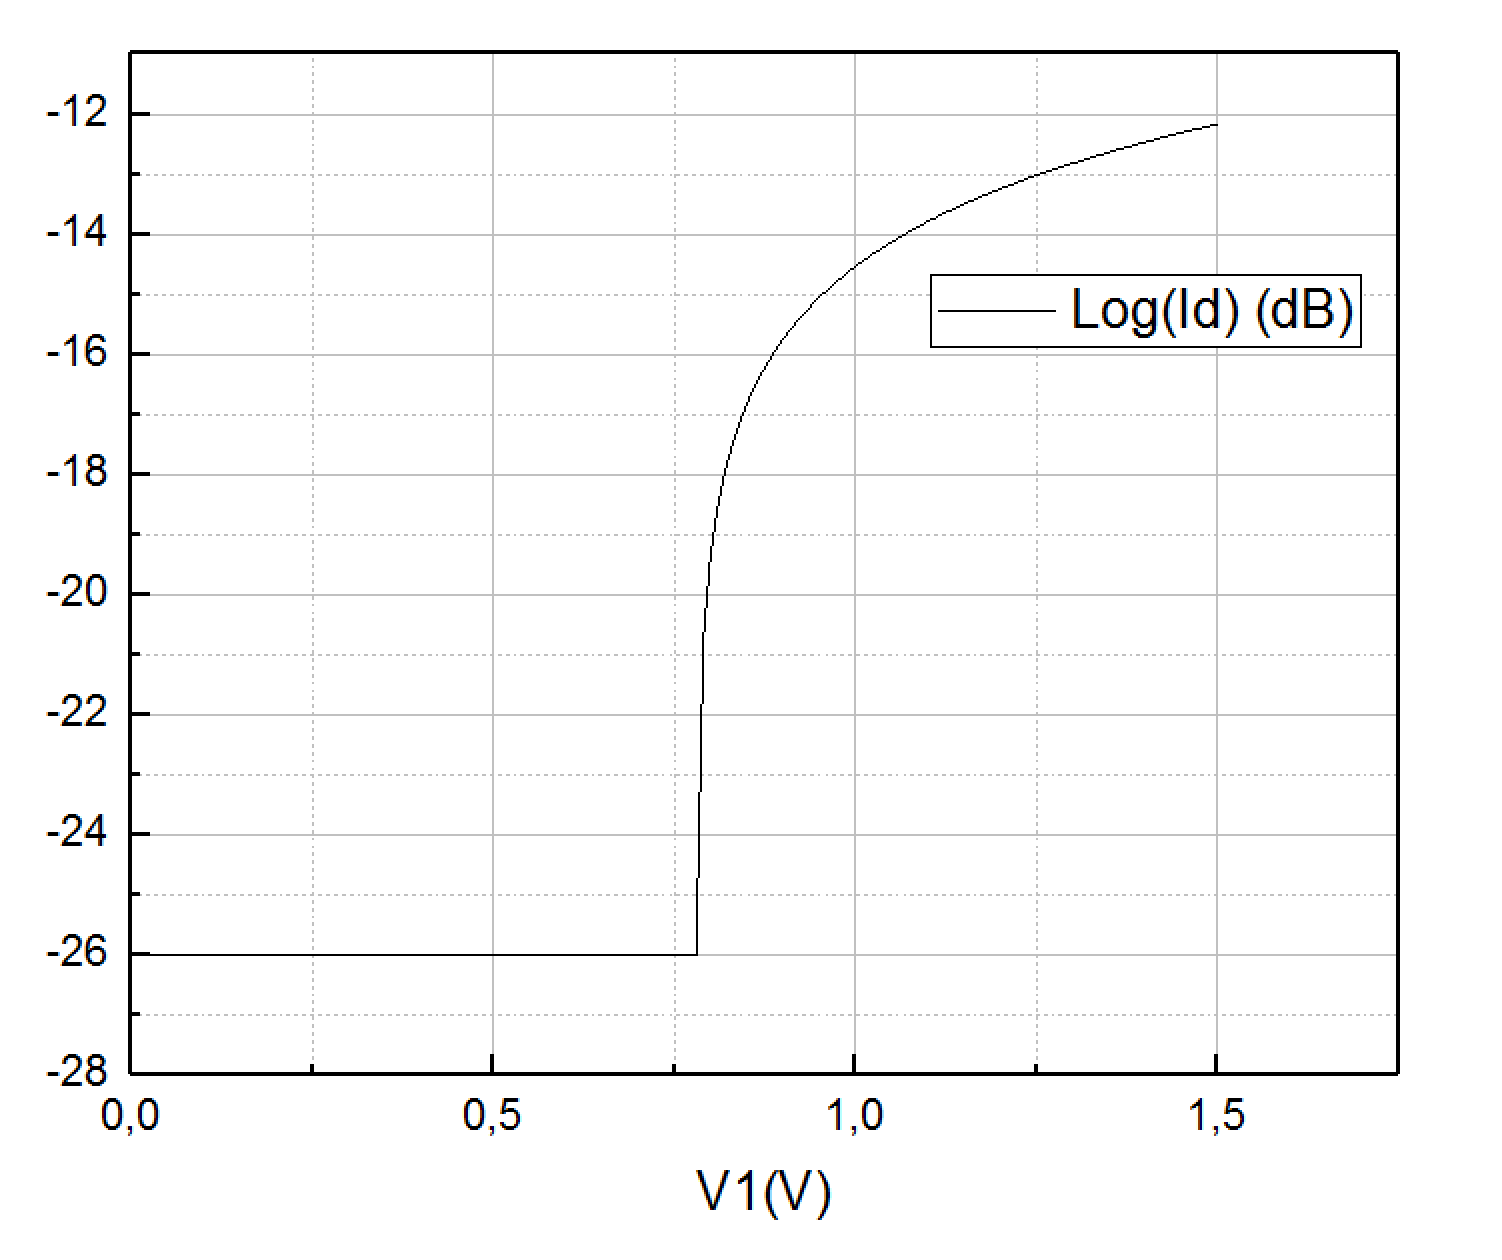
\includegraphics[width=6cm]{Imagenes/Sinaptico/Polariz_sim_malo}}
		\subfigure[Modelo Level 3 completo]{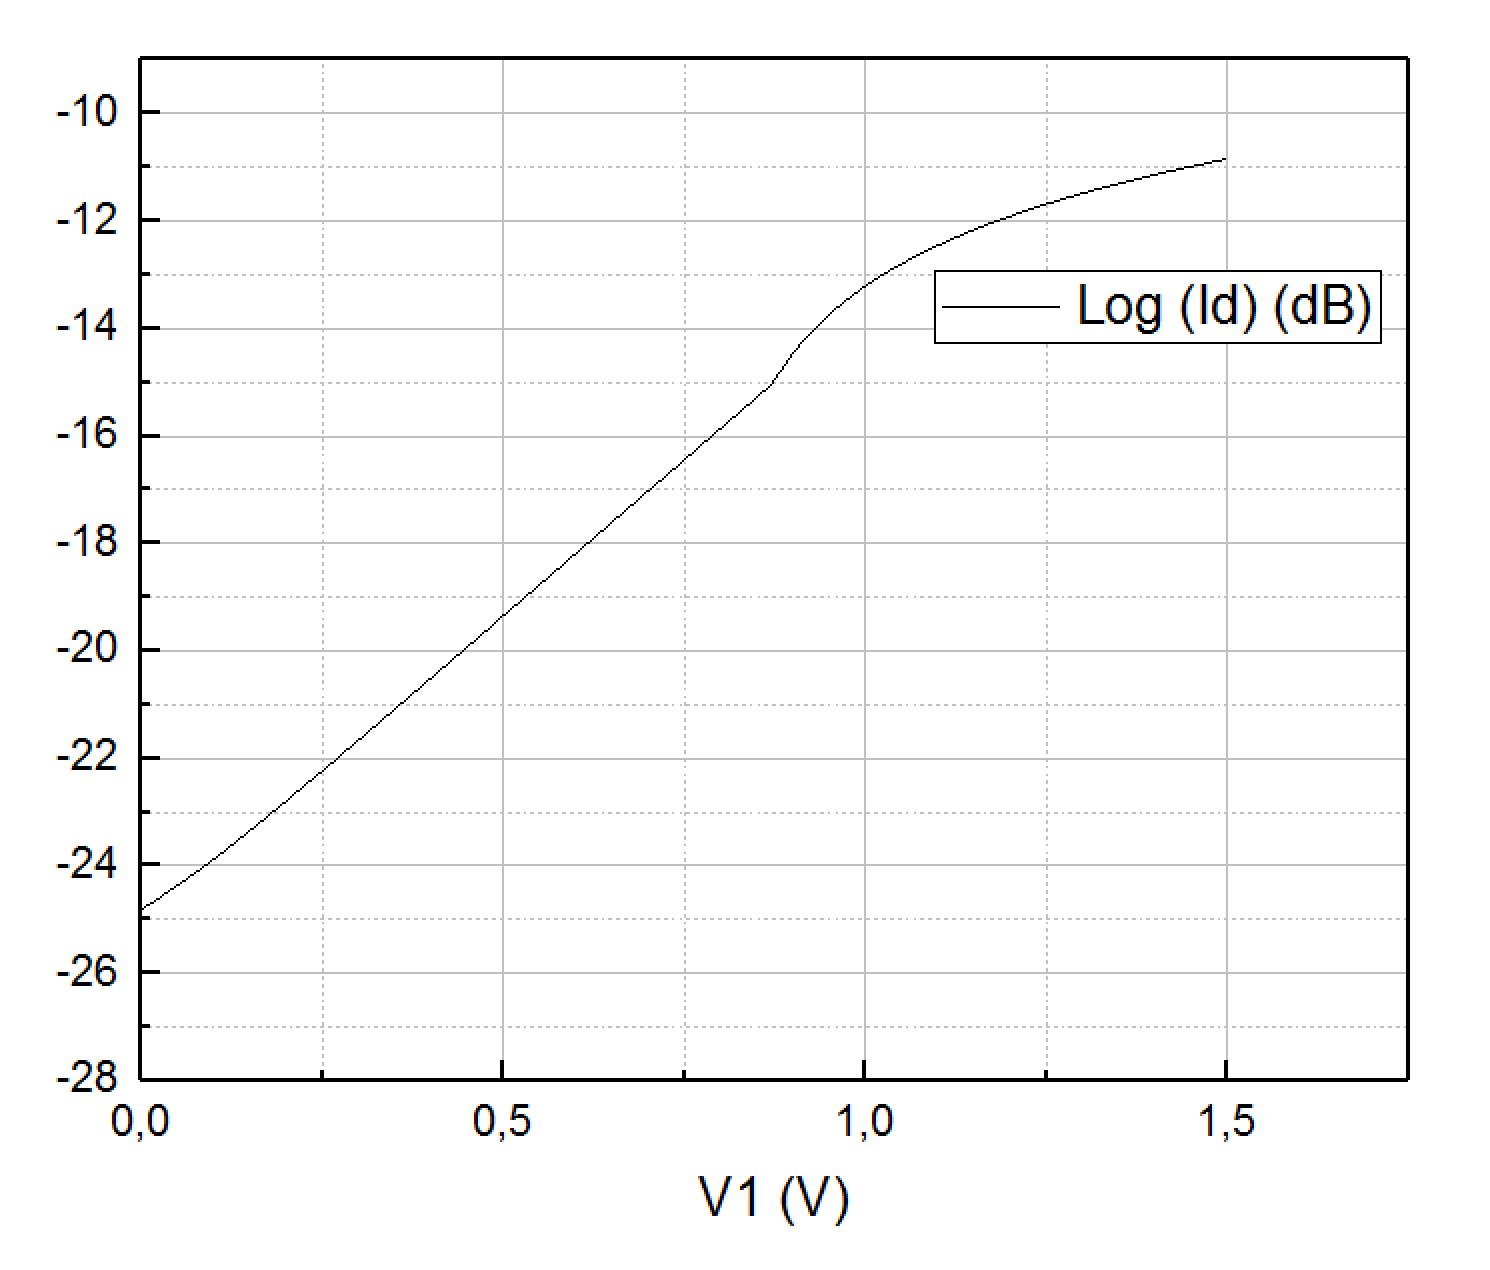
\includegraphics[width=6cm]{Imagenes/Sinaptico/Polariz_sim}}
		\caption{Corriente a través de $M1$ frente a $V_1$}	\label{Polariz_sim}
	\end{figure}
	
	En la figura \ref{Polariz_sim} se muestra el resultado obtenido. Hasta que $V_{GS}>V_T$, el resultado para el modelo básico Level 1 es una constante, mientras que para el modelo más completo Level 3 es una recta, que es el resultado de aplicar el logaritmo a la ecuación de la corriente 5.4. Por tanto se tomará el modelo Level 3 para representa correctamente lo que ocurre en la región subumbral. Este modelo será el que se use para el resto de simulaciones.
	
	\subsection{Modelo inicial}
	
	\subsubsection{Análisis en frecuencia}
	
	A continuación se va a simular el modelo de circuito inicial de la figura \ref{Inicial}. En primer lugar se hará un análisis en el dominio de la frecuencia. Para observar la variación que produce la corriente $I_{\tau}$ en la frecuencia de corte del circuito, se ha hecho una simulación paramétrica en la que se ha variado iterativamente el valor de esta corriente. El resultado se muestra en la figura \ref{Frecuencia_Corte}.
	
	
    \begin{center}
		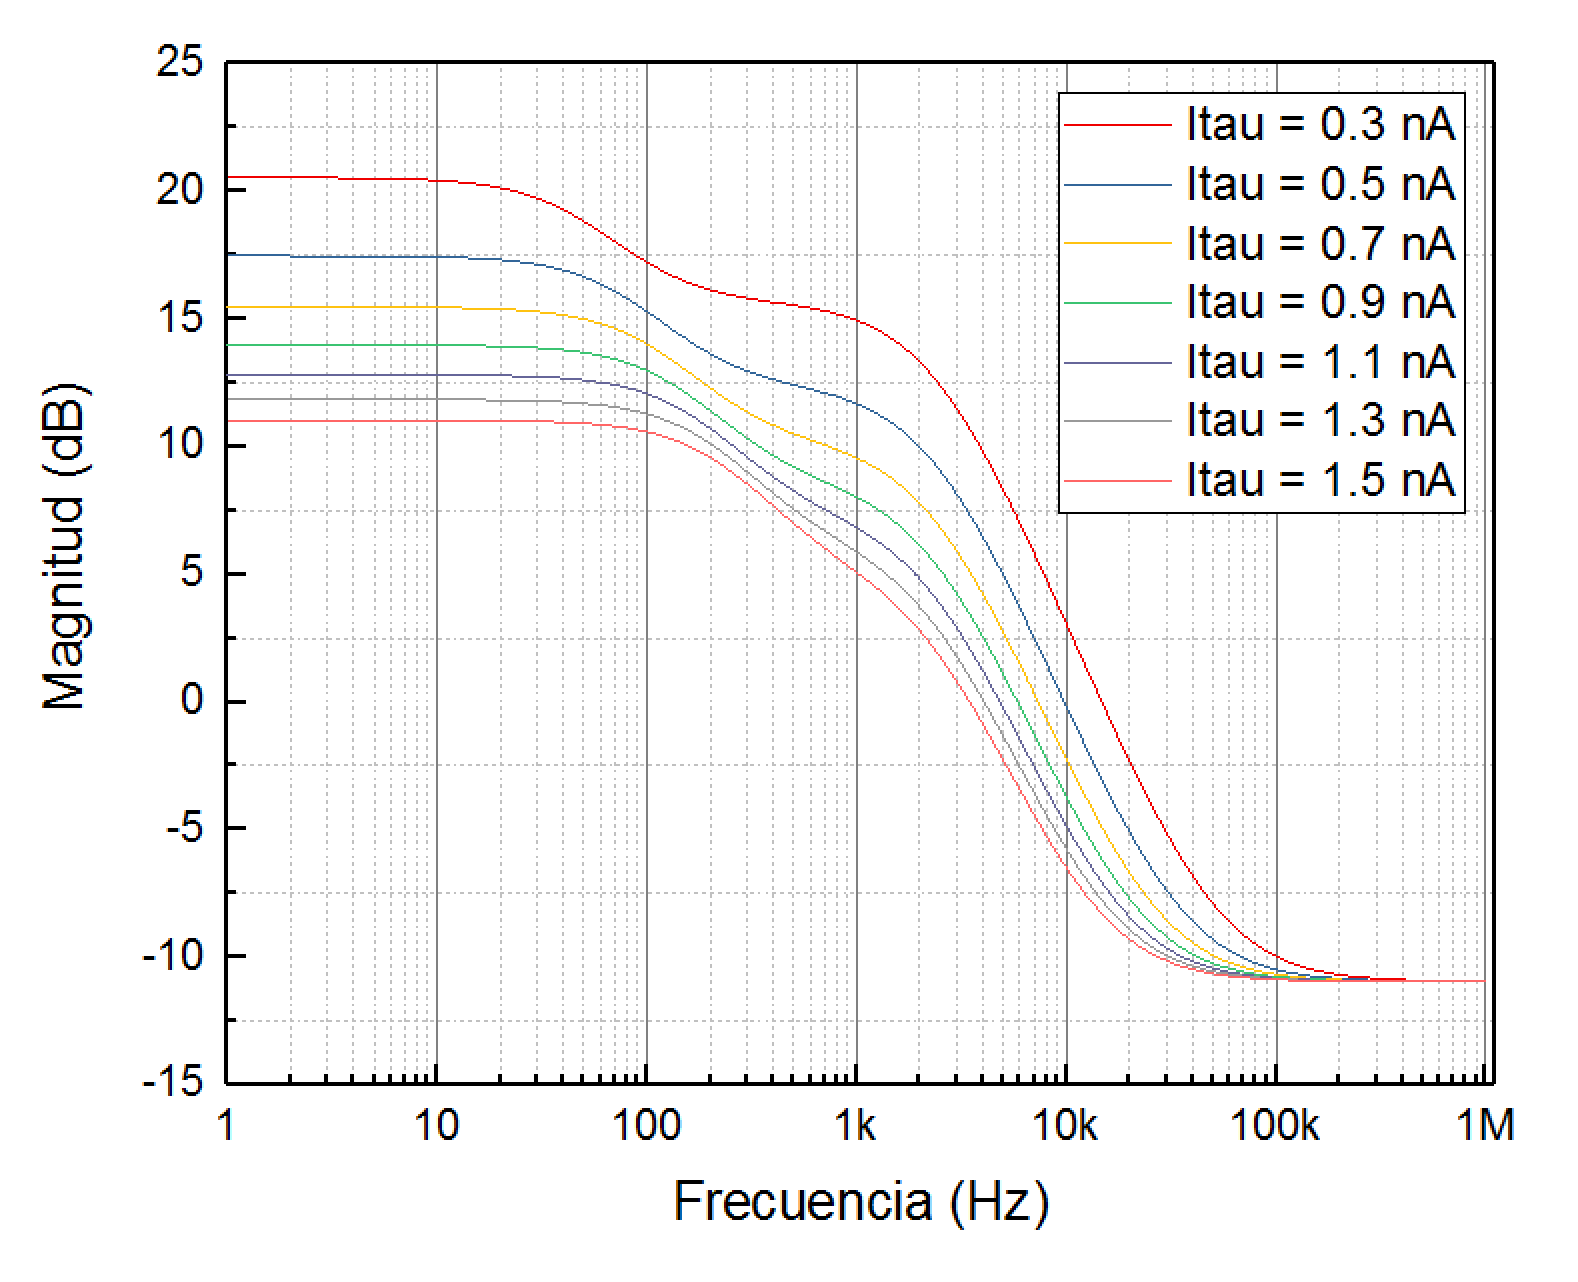
\includegraphics[width=12cm]{Imagenes/Sinaptico/Inicial_Itau}
    		\captionof{figure}{Frecuencia de corte para distintos valores de $I_{\tau}$}\label{Frecuencia_Corte}
	\end{center}	
	
	Se observa que conforme aumenta el valor de la corriente $I_{\tau}$ aumenta la frecuencia de corte al mismo tiempo que disminuye la ganancia. Esto se debe a que en la función de transferencia del circuito, la ganancia es el factor $\frac{I_g^P}{I_{\tau}}$, por tanto conforme $I_{\tau}$ aumenta, la ganancia disminuye. El aumento de la frecuencia de corte es una consecuencia directa de que $\tau$ disminuye.
	
		\begin{center}
		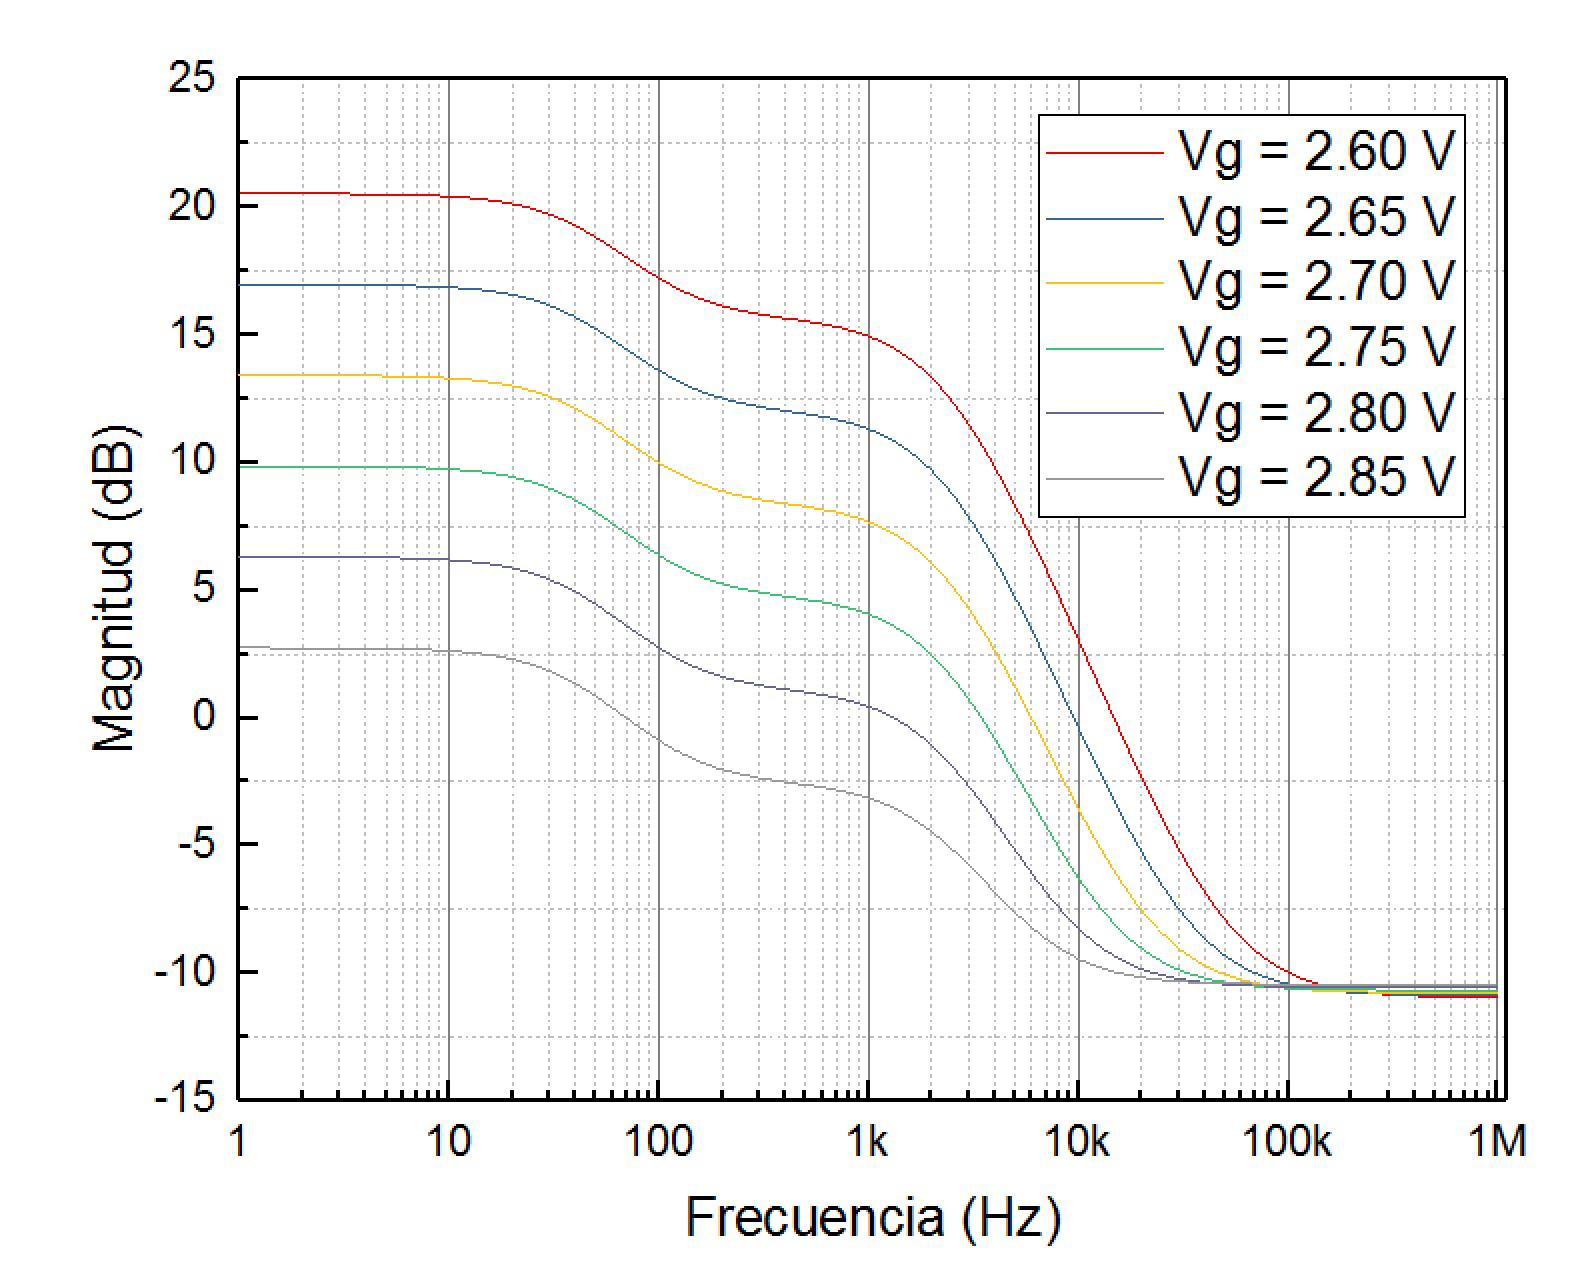
\includegraphics[width=12cm]{Imagenes/Sinaptico/Inicial_Vg}
    		\captionof{figure}{Esquemático del circuito de polarización}\label{Inicial_Vg}
	\end{center}	
	
	En la figura \ref{Inicial_Vg} se ha mantenido constante el valor de $I_{tau}$ y se ha variado el valor de $V_g$. Se observa que en este caso el único parámetro que se ve alterado es la ganancia del circuito, mientras que la frecuencia de corte es la misma para los distintos valores de $V_g$. Obsérvese que conforme aumenta el valor de $V_g$, disminuye la ganancia del circuito. Recuérdese que:
	
	$$I_g^P=I_0e^{\frac{\kappa}{V_T}(V_{dd}-V_g)}$$ y que en la función de transferencia del circuito, la ganancia es el factor $\frac{I_g^P}{I_{\tau}}$. De forma que cuando $V_g$ aumenta, la exponencial se hace más pequeña, disminuyendo así el valor de $I_g^P$ y por tanto la ganancia del circuito.
	
	\subsubsection{Análisis en el tiempo}
	
		
	\begin{center}
		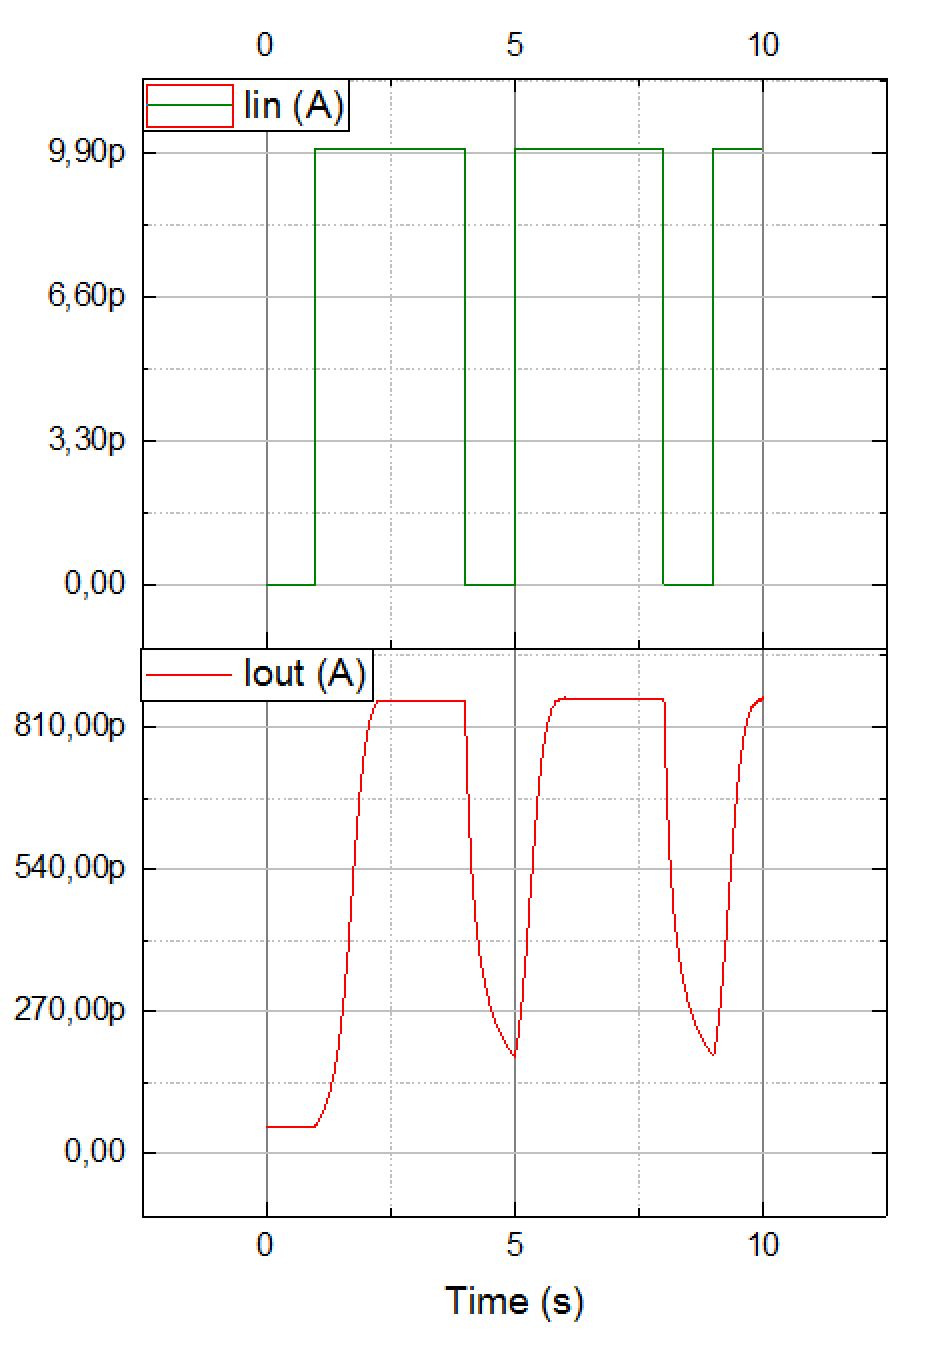
\includegraphics[width=8cm]{Imagenes/Sinaptico/Inicial_time}
    		\captionof{figure}{Salida para una entrada de pulsos cuadrados}\label{Inicial_time}
	\end{center}	
	
	En la figura \ref{Inicial_time} se muestra la salida $I_{out}$ para una entrada de pulsos cuadrados. Cuando la señal cuadrada pasa de un nivel bajo a un nivel alto, se observa a la salida la fase de carga que se esperaba tras el análisis teórico mostrado. Cuando pasa de un nivel alto a uno bajo, se produce la fase de descarga.
	
	\subsection{Modelo Completo}

A continuación se muestran las simulaciones realizadas para el circuito completo, cuyo esquemático se muestra en la figura \ref{Segundo}.

\subsubsection{Análisis en frecuencia}

Los resultados obtenidos en la simulación en frecuencia del circuito completo son idénticos a los obtenidos con el modelo más simple. Las únicas diferencias han sido que en este caso el valor de la corriente $I_{\tau}$ que antes se controlaba mediante una fuente de corriente ideal, ahora se ha controlado mediante la tensión de puerta $V_{\tau}$ del transistor que sustituye a esta fuente de corriente. En cualquier caso la conclusión es la misma: variando la corriente $I_{\tau}$ varía tanto la ganancia de forma lineal, como la frecuencia de corte; variando $V_g$ varía la ganancia exponencialmente.

\subsubsection{Análisis en el tiempo}

En cuanto al análisis temporal, se han obtenido de nuevo los mismos resultados que en el caso del modelo con las fuentes de corriente simplificadas. Se ha probado a variar el valor de la capacidad del circuito para ver cómo afectaba a la constante de tiempo del circuito.

	\begin{center}
		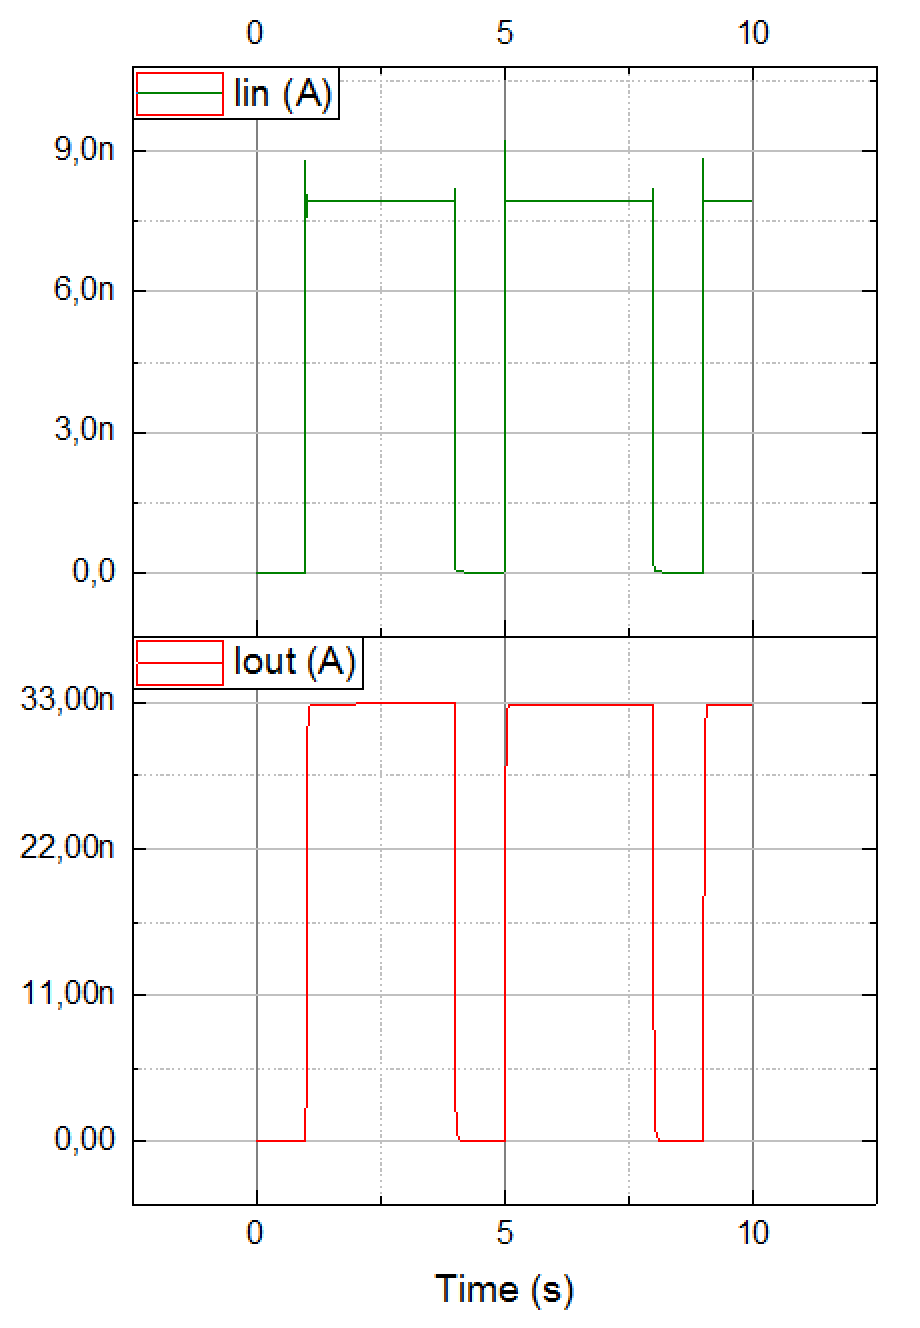
\includegraphics[width=9.5cm]{Imagenes/Sinaptico/Segundo_time}
    		\captionof{figure}{Salida del circuito completo para una entrada de pulsos cuadrados}\label{Segundo_time}
	\end{center}	
	
	En la figura \ref{Segundo_time} se observa que al haber variado el valor del condensador, el paso de un valor bajo a uno alto de la señal de salida es muy rápido. Por tanto el valor de la capacidad es otro de los parámetros a tener en cuenta.

\section{Modelo extendido}

En el modelo propuesto hasta ahora se puede observar en base a los resultados obtenidos de la simulación como la respuesta del circuito modela la corriente sináptica generada por una excitación sináptica. Sin embargo, se pueden añadir otros circuitos al mostrado para añadir nuevas características propias de las sinapsis biológicas. Esto se muestra en la figura \ref{Final}. La parte de color verde añade el comportamiento de los receptores sinápticos NMDA. Estos hacen que la corriente iónica fluya solo si la membrana está polarizada a una tensión superior a una de corte, en presencia de los neurotransmisores. Este comportamiento es replicable haciendo uso de nuevo del par diferencial, de forma que cuando la tensión en el nodo $V_{mem}$ es menor que la tensión $V_{nmda}$, la corriente de salida circula solo por la rama de la izquieda y por tanto no tiene ningún efecto en la corriente final de salida del circuito. En caso contrario, la corriente circula por ambas ramas de forma que se consigue la implementación de la sinapsis NMDA. 

Por otra parte, la parte de color rojo corresponde a la parte que se encarga de añadir plasticidad al circuito. Con el modelo inicial se ha conseguido llegar a reproducir dinámicas de corrientes sinápticas reales. Sin embargo una de las funciones principales de las redes neuronales es la plasticidad, esto es, la capacidad de aprender y adaptarse al entorno. Para conseguir esto se ha hecho uso del circuito propuesto por Rasche y Hahnloser en 2001 \cite{rasche2001silicon}. Este circuito se puede describir como un mecanismo no lineal que juega un papel fundamental para implementar selectividad en estímulos transitorios y adaptación. En la figura \ref{Neurona} se muestra la corriente de salida al aplicar un pulso a la entrada. Se observa como los picos de salida van disminuyendo poco a poco a partir del tercero de ellos. Esto demuestra que el circuito se acostumbra al impulso recibido.

	\begin{center}
		\includegraphics[width=12cm]{Imagenes/Sinaptico/Final_2.eps}
    		\captionof{figure}{Esquemático del circuito ampliado}\label{Final}
	\end{center}	
	
		\begin{center}
		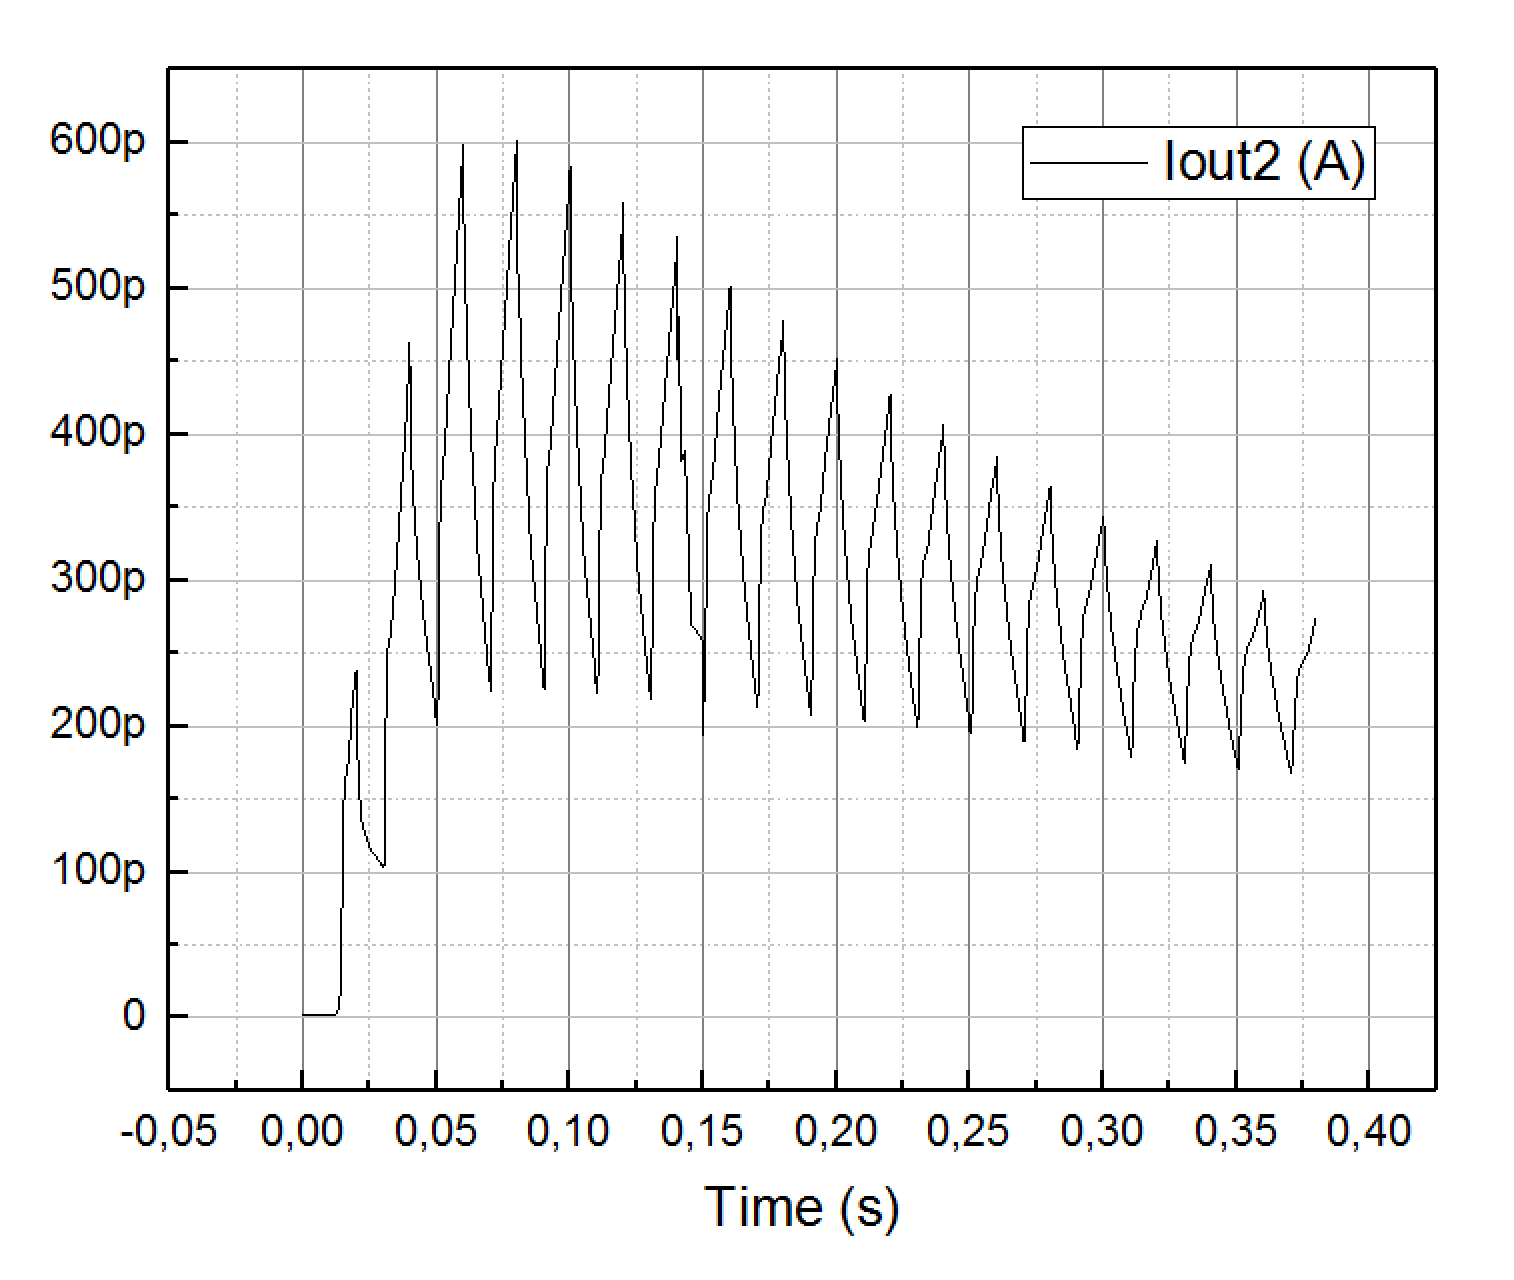
\includegraphics[width=10cm]{Imagenes/Sinaptico/Neurona}
    		\captionof{figure}{Respuesta del sistema a un tren de impulsos}\label{Neurona}
	\end{center}	
	
	



